\documentclass{article}

\usepackage{tikz}

\begin{document}
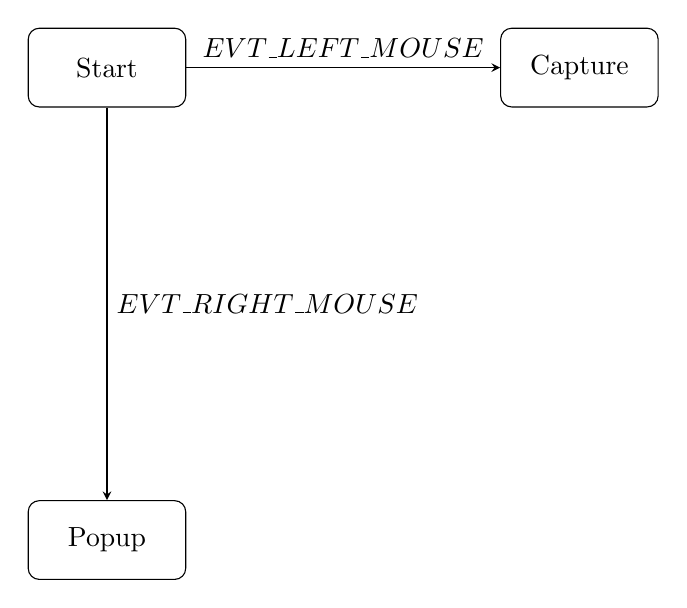
\begin{tikzpicture}
%define
\tikzstyle{state} = [rectangle, rounded corners, minimum width=2cm, minimum height=1cm, text centered, draw=black]
\tikzstyle{arrow} = [->, >=stealth]

\node[state, draw, align=left](start){Start};
\node[state, right of = start, xshift = 5cm, draw, align=left](state_Capture){Capture};
\node[state, below of = start, yshift = -5cm, draw, align=left](state_Popup){Popup};

\draw[arrow](start) -- node[above]{$EVT\_LEFT\_MOUSE$}(state_Capture);
\draw[arrow](start) -- node[right]{$EVT\_RIGHT\_MOUSE$}(state_Popup);

\end{tikzpicture}
\end{document}